% 图 22.4 —— 由 `checks/emit_hand.py` 自动拼出（probe 精测 + prims2 图元分解）
%%
% ⚠ 这是**稿子不是成品**：跑 `checks/checkhand.py 22.4` 看指标 + 看叠合图。
%%
%% ⚠ 待核：
%   · 本图 probe 报出阴影族 4 个 —— **本脚本不生成阴影**（要照原书手写）；prims2 的 strokes 里可能含阴影线，核对时留意别画重
%   · 可疑字形 3 项（空心圈 ⊙ 常被认成字母 o）—— 见文件末
%%
\documentclass[12pt]{standalone}
\usepackage{fontspec}
\setsansfont{Arial}
\newfontfamily\mfallback{DejaVu Sans}
\usepackage{tikz}
\begin{document}
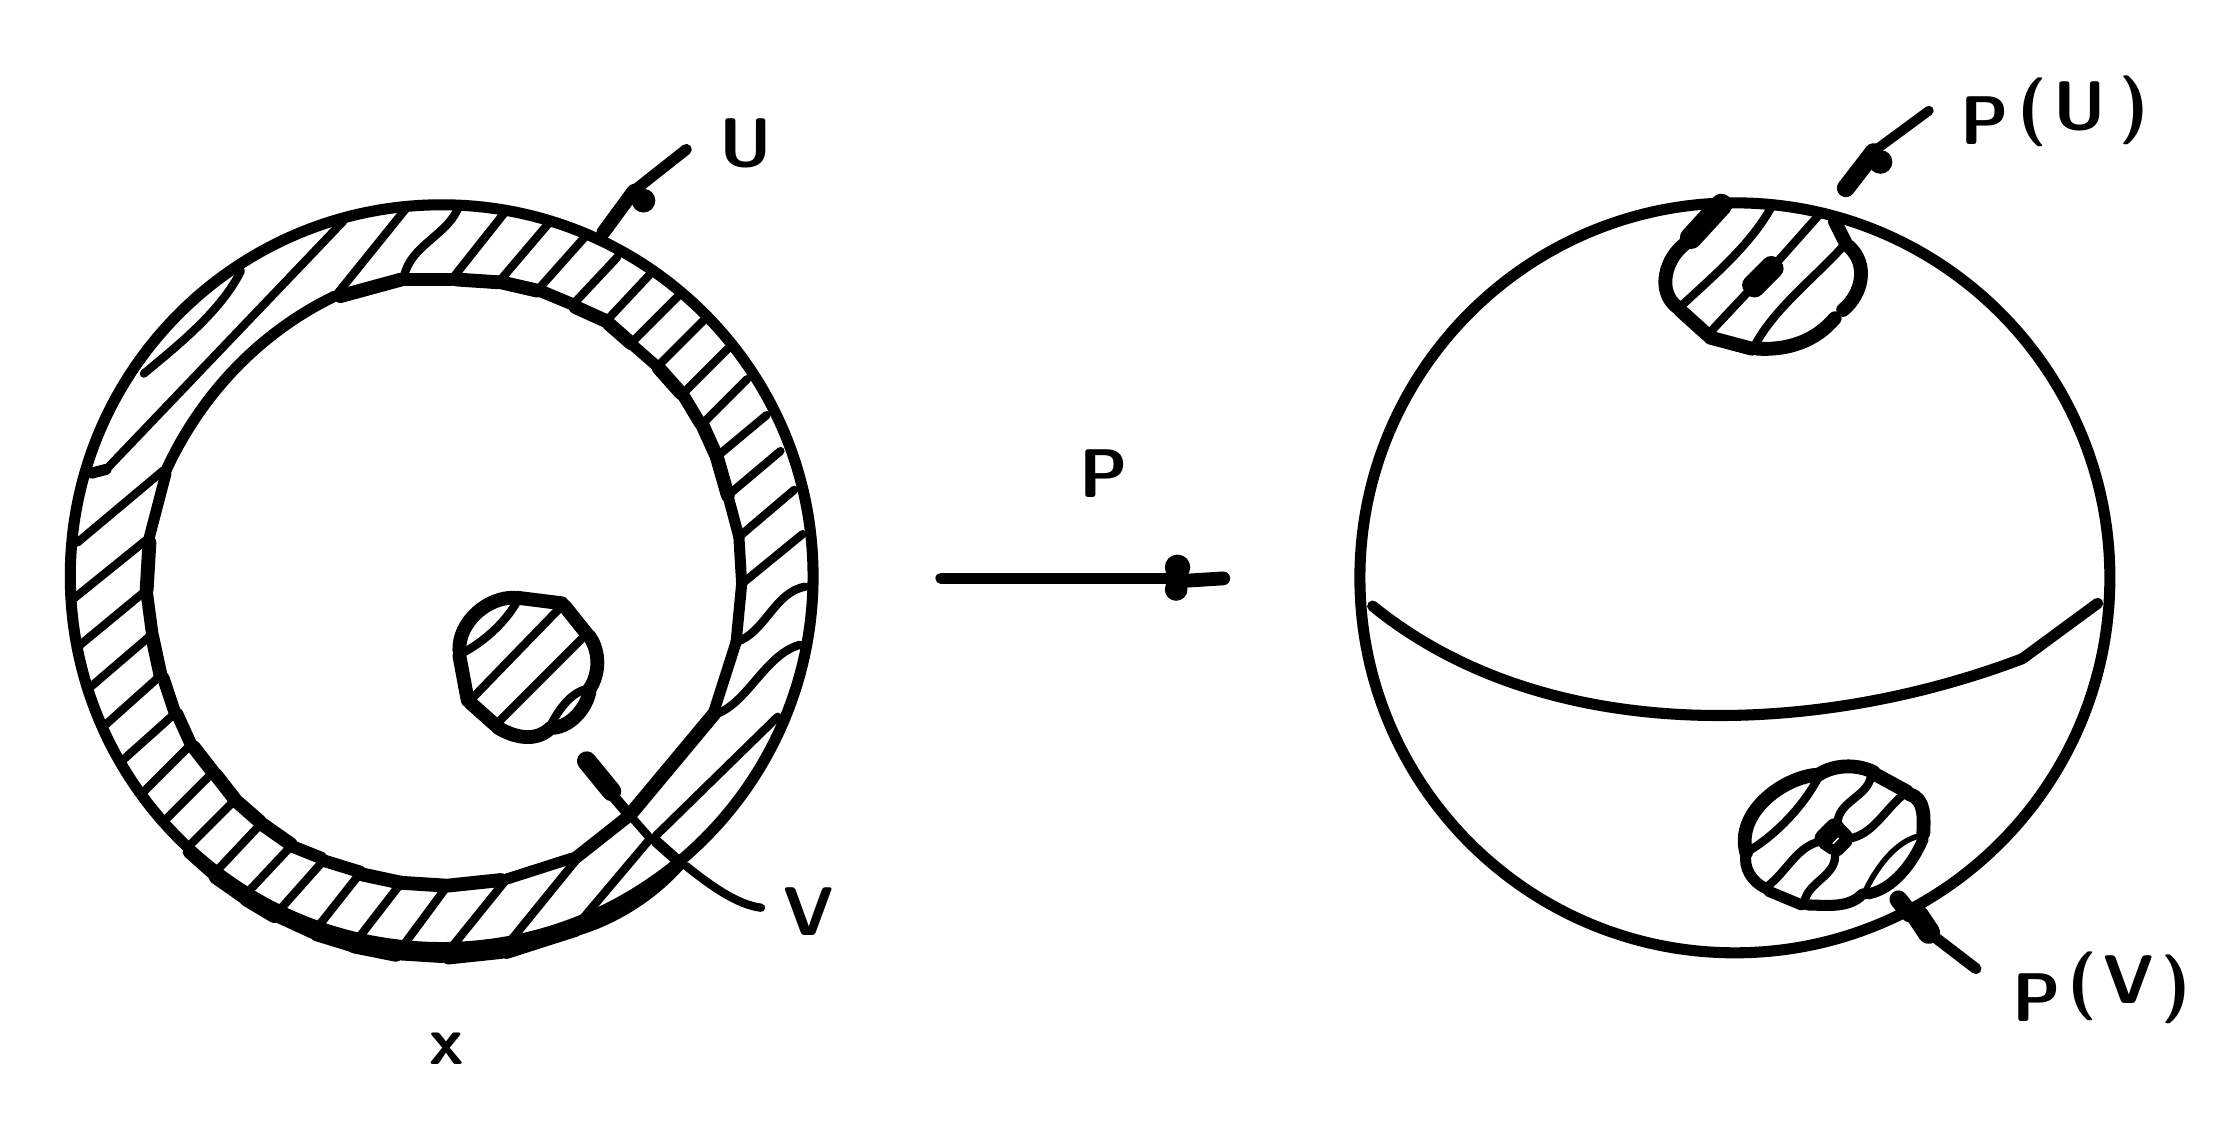
\begin{tikzpicture}[x=1pt, y=-1pt, line width=4.0pt, line cap=round, line join=round]

  %% ════ 填充区（prims2 的 fills）════

  %% ════ 直线段（prims2 的 strokes）════
  \draw[line width=6.5pt] (657.0,58.0) -- (667.0,45.0);
  \draw[line width=5.0pt] (228.0,123.0) -- (236.0,132.0);
  \draw[line width=3.0pt] (154.0,90.0) -- (173.0,66.0);
  \draw[line width=5.0pt] (155.0,91.0) -- (170.0,92.0);
  \draw[line width=3.0pt] (267.0,140.0) -- (249.0,155.0);
  \draw[line width=4.5pt] (237.0,133.0) -- (243.0,143.0);
  \draw[line width=4.0pt] (219.0,115.0) -- (227.0,122.0);
  \draw[line width=4.7pt] (657.0,292.0) -- (654.0,289.0);
  \draw[line width=3.0pt] (225.0,293.0) -- (218.0,285.0);
  \draw[line width=3.0pt] (225.0,293.0) -- (198.0,325.0);
  \draw[line width=3.0pt] (90.0,320.0) -- (106.0,302.0);
  \draw[line width=5.0pt] (152.0,310.0) -- (171.0,308.0);
  \draw[line width=3.0pt] (172.0,333.0) -- (198.0,301.0);
  \draw[line width=4.0pt] (330.0,199.0) -- (413.0,199.0);
  \draw[line width=3.0pt] (119.0,307.0) -- (104.0,326.0);
  \draw[line width=3.0pt] (112.0,96.0) -- (137.0,65.0);
  \draw[line width=5.0pt] (218.0,114.0) -- (210.0,107.0);
  \draw[line width=5.0pt] (416.0,200.0) -- (432.0,199.0);
  \draw[line width=5.0pt] (136.0,91.0) -- (153.0,91.0);
  \draw[line width=4.0pt] (44.0,184.0) -- (50.0,161.0);
  \draw[line width=4.5pt] (96.0,296.0) -- (106.0,300.0);
  \draw[line width=4.0pt] (150.0,336.0) -- (134.0,335.0);
  \draw[line width=8.1pt] (683.0,321.0) -- (687.0,327.0);
  \draw[line width=5.0pt] (607.0,111.0) -- (597.0,102.0);
  \draw[line width=5.0pt] (151.0,310.0) -- (135.0,309.0);
  \draw[line width=5.0pt] (43.0,203.0) -- (44.0,186.0);
  \draw[line width=5.0pt] (169.0,252.0) -- (160.0,244.0);
  \draw[line width=3.0pt] (271.0,249.0) -- (227.0,292.0);
  \draw[line width=4.0pt] (238.0,44.0) -- (219.0,59.0);
  \draw[line width=3.0pt] (68.0,305.0) -- (84.0,288.0);
  \draw[line width=5.0pt] (171.0,92.0) -- (184.0,95.0);
  \draw[line width=3.0pt] (49.0,160.0) -- (18.0,186.0);
  \draw[line width=4.0pt] (23.0,161.0) -- (28.4,159.6);
  \draw[line width=3.0pt] (28.4,159.6) -- (114.0,70.0);
  \draw[line width=5.0pt] (194.0,209.0) -- (202.0,219.0);
  \draw[line width=4.5pt] (54.0,248.0) -- (59.0,259.0);
  \draw[line width=4.0pt] (720.8,228.0) -- (748.0,208.0);
  \draw[line width=4.0pt] (211.0,277.0) -- (217.0,284.0);
  \draw[line width=5.0pt] (679.0,276.0) -- (668.0,270.0);
  \draw[line width=5.0pt] (198.0,326.0) -- (173.0,334.0);
  \draw[line width=4.5pt] (185.0,95.0) -- (197.0,100.0);
  \draw[line width=5.0pt] (121.0,306.0) -- (135.0,309.0);
  \draw[line width=7.0pt] (630.0,86.0) -- (623.0,93.0);
  \draw[line width=3.0pt] (253.0,116.0) -- (237.0,132.0);
  \draw[line width=3.0pt] (58.0,296.0) -- (74.0,280.0);
  \draw[line width=6.5pt] (680.0,320.0) -- (676.0,315.0);
  \draw[line width=7.0pt] (624.0,94.0) -- (631.0,87.0);
  \draw[line width=5.0pt] (113.0,97.0) -- (135.0,91.0);
  \draw[line width=5.0pt] (67.0,269.0) -- (60.0,260.0);
  \draw[line width=5.0pt] (249.0,155.0) -- (244.0,144.0);
  \draw[line width=5.0pt] (249.0,155.0) -- (253.0,169.0);
  \draw[line width=5.0pt] (68.0,270.0) -- (75.0,279.0);
  \draw[line width=4.0pt] (256.0,222.0) -- (258.0,201.0);
  \draw[line width=4.0pt] (256.0,222.0) -- (248.0,247.0);
  \draw[line width=4.0pt] (687.0,327.0) -- (704.0,340.0);
  \draw[line width=5.0pt] (657.0,78.0) -- (653.0,70.0);
  \draw[line width=3.0pt] (28.0,252.0) -- (47.0,235.0);
  \draw[line width=4.5pt] (120.0,305.0) -- (107.0,301.0);
  \draw[line width=3.0pt] (172.0,309.0) -- (151.0,335.0);
  \draw[line width=4.0pt] (257.0,184.0) -- (253.0,169.0);
  \draw[line width=3.0pt] (257.0,184.0) -- (277.0,167.0);
  \draw[line width=4.0pt] (257.0,184.0) -- (258.0,201.0);
  \draw[line width=5.0pt] (85.0,288.0) -- (95.0,295.0);
  \draw[line width=4.5pt] (53.0,247.0) -- (49.0,235.0);
  \draw[line width=5.0pt] (218.0,284.0) -- (248.0,248.0);
  \draw[line width=3.0pt] (44.0,220.0) -- (23.0,238.0);
  \draw[line width=5.0pt] (78.0,314.0) -- (68.0,307.0);
  \draw[line width=3.0pt] (225.0,89.0) -- (210.0,105.0);
  \draw[line width=3.0pt] (219.0,113.0) -- (235.0,97.0);
  \draw[line width=5.0pt] (84.0,287.0) -- (76.0,280.0);
  \draw[line width=5.0pt] (133.0,335.0) -- (118.0,332.0);
  \draw[line width=3.5pt] (687.0,30.0) -- (668.0,44.0);
  \draw[line width=3.0pt] (135.0,309.0) -- (118.0,331.0);
  \draw[line width=4.0pt] (641.0,317.0) -- (629.0,312.0);
  \draw[line width=5.0pt] (198.0,101.0) -- (209.0,106.0);
  \draw[line width=4.5pt] (90.0,321.0) -- (103.0,327.0);
  \draw[line width=4.7pt] (654.0,297.0) -- (657.0,294.0);
  \draw[line width=4.0pt] (117.0,332.0) -- (104.0,328.0);
  \draw[line width=5.0pt] (608.0,112.0) -- (623.0,116.0);
  \draw[line width=5.0pt] (208.0,74.0) -- (219.0,59.0);
  \draw[line width=3.0pt] (258.0,201.0) -- (280.0,183.0);
  \draw[line width=6.7pt] (653.0,289.0) -- (649.0,293.0);
  \draw[line width=3.0pt] (43.0,185.0) -- (17.0,206.0);
  \draw[line width=3.0pt] (244.0,106.0) -- (228.0,122.0);
  \draw[line width=5.0pt] (89.0,321.0) -- (79.0,315.0);
  \draw[line width=5.0pt] (48.0,234.0) -- (45.0,220.0);
  \draw[line width=3.0pt] (151.0,311.0) -- (134.0,334.0);
  \draw[line width=4.5pt] (43.0,204.0) -- (45.0,219.0);
  \draw[line width=5.0pt] (156.0,227.0) -- (159.0,243.0);
  \draw[line width=3.0pt] (53.0,248.0) -- (34.0,265.0);
  \draw[line width=5.0pt] (177.0,206.0) -- (193.0,208.0);
  \draw[line width=3.0pt] (19.0,223.0) -- (42.0,204.0);
  \draw[line width=3.0pt] (49.0,287.0) -- (66.0,270.0);
  \draw[line width=5.0pt] (152.0,336.0) -- (171.0,334.0);
  \draw[line width=3.0pt] (192.0,210.0) -- (160.0,243.0);
  \draw[line width=4.5pt] (198.0,300.0) -- (217.0,285.0);
  \draw[line width=3.0pt] (623.0,94.0) -- (608.0,110.0);
  \draw[line width=3.0pt] (201.0,220.0) -- (170.0,251.0);
  \draw[line width=3.0pt] (94.0,297.0) -- (79.0,313.0);
  \draw[line width=3.8pt] (649.0,295.0) -- (652.0,297.0);
  \draw[line width=8.0pt] (601.0,76.0) -- (612.0,64.0);
  \draw[line width=3.0pt] (201.0,76.0) -- (185.0,94.0);
  \draw[line width=3.0pt] (260.0,127.0) -- (244.0,143.0);
  \draw[line width=3.0pt] (198.0,99.0) -- (213.0,83.0);
  \draw[line width=4.0pt] (197.0,300.0) -- (172.0,308.0);
  \draw[line width=3.0pt] (253.0,169.0) -- (272.0,153.0);
  \draw[line width=7.0pt] (202.0,265.0) -- (211.0,276.0);
  \draw[line width=3.0pt] (171.0,91.0) -- (188.0,71.0);
  \draw[line width=3.0pt] (41.0,277.0) -- (58.0,260.0);
  \draw[line width=3.0pt] (631.0,86.0) -- (647.0,68.0);
  \draw[line width=4.0pt] (67.0,306.0) -- (58.0,298.0);
  \draw[line width=4.0pt] (236.0,302.0) -- (227.0,294.0);

  %% ════ 曲线（prims2 的 curves —— 三段式，坐标同为 (y,x)）════
  \draw[line width=3.0pt] (624.0,115.0) .. controls (631.2,101.4) and (645.2,90.9) .. (656.0,79.0);
  \draw[line width=5.0pt] (647.0,270.0) .. controls (652.7,266.2) and (661.0,266.0) .. (667.0,269.0);
  \draw[line width=3.0pt] (177.0,207.0) .. controls (172.8,214.8) and (164.8,222.0) .. (157.0,226.0);
  \draw[line width=5.0pt] (189.0,253.0) .. controls (183.5,258.4) and (175.8,256.4) .. (170.0,253.0);
  \draw[line width=2.0pt] (684.0,292.0) .. controls (674.9,293.6) and (667.6,304.3) .. (664.0,312.0);
  \draw[line width=5.0pt] (646.0,270.0) .. controls (633.4,271.4) and (617.2,284.1) .. (621.0,298.0);
  \draw[line width=3.0pt] (654.0,288.0) .. controls (653.7,279.8) and (664.3,278.2) .. (666.0,271.0);
  \draw[line width=3.0pt] (238.0,303.0) .. controls (245.9,309.3) and (256.0,316.9) .. (265.0,318.0);
  \draw[line width=4.0pt] (628.0,311.0) .. controls (623.0,308.6) and (619.8,303.7) .. (621.0,298.0);
  \draw[line width=5.0pt] (203.0,220.0) .. controls (206.8,225.4) and (206.8,233.4) .. (203.0,239.0);
  \draw[line width=5.0pt] (156.0,225.0) .. controls (155.6,214.9) and (166.1,205.6) .. (176.0,206.0);
  \draw[line width=4.0pt] (486.0,209.0) .. controls (549.7,260.7) and (647.9,255.8) .. (720.8,228.0);
  \draw[line width=3.0pt] (202.0,239.0) .. controls (196.1,240.3) and (191.7,246.8) .. (189.0,252.0);
  \draw[line width=5.0pt] (653.0,105.0) .. controls (645.8,113.5) and (635.8,116.6) .. (625.0,116.0);
  \draw[line width=4.0pt] (643.0,317.0) .. controls (649.1,317.0) and (658.0,318.5) .. (663.0,313.0);
  \draw[line width=5.0pt] (203.0,240.0) .. controls (201.8,245.9) and (196.4,252.4) .. (190.0,253.0);
  \draw[line width=4.0pt] (685.0,293.0) .. controls (681.6,301.3) and (674.3,311.4) .. (665.0,313.0);
  \draw[line width=3.0pt] (256.0,222.0) .. controls (266.5,218.7) and (269.9,203.8) .. (281.0,202.0);
  \draw[line width=3.0pt] (629.0,310.0) .. controls (635.7,304.8) and (639.5,295.6) .. (648.0,294.0);
  \draw[line width=3.0pt] (249.0,248.0) .. controls (260.7,243.3) and (266.5,226.6) .. (279.0,223.0);
  \draw[line width=3.0pt] (647.0,271.0) .. controls (641.5,281.6) and (631.0,292.4) .. (621.0,298.0);
  \draw[line width=5.0pt] (680.0,277.0) .. controls (685.9,278.7) and (685.1,285.9) .. (685.0,291.0);
  \draw[line width=5.0pt] (656.0,102.0) .. controls (663.0,96.2) and (665.3,85.4) .. (658.0,79.0);
  \draw[line width=3.0pt] (630.0,65.0) .. controls (622.2,78.8) and (609.1,89.8) .. (597.0,101.0);
  \draw[line width=3.0pt] (136.0,90.0) .. controls (138.2,78.4) and (152.5,74.8) .. (156.0,64.0);
  \draw[line width=3.0pt] (77.0,88.0) .. controls (69.7,102.6) and (54.0,115.0) .. (42.0,125.0);
  \draw[line width=4.0pt] (111.0,97.0) .. controls (84.0,110.0) and (62.6,132.5) .. (50.0,160.0);
  \draw[line width=3.0pt] (653.0,298.0) .. controls (654.3,306.4) and (643.2,308.4) .. (642.0,316.0);
  \draw[line width=4.0pt] (199.0,326.0) .. controls (212.8,321.8) and (226.3,313.1) .. (236.0,302.0);
  \draw[line width=5.0pt] (596.0,101.0) .. controls (588.4,94.9) and (592.0,83.1) .. (599.0,78.0);
  \draw[line width=3.0pt] (678.0,277.0) .. controls (671.3,282.2) and (666.6,292.0) .. (658.0,293.0);

  %% ════ 圆 / 椭圆（probe 精测）════
  \draw (616.9,198.8) circle (135.5);
  \draw (149.6,198.2) circle (134.2);

  %% ════ 实心点 ════
  \fill (669.5,48.5) circle (4.3);
  \fill (222.5,62.5) circle (4.3);
  \fill (415.5,195.0) circle (4.6);
  \fill (415.0,203.0) circle (4.1);

  %% ════ 标签（probe 直接给的 \node 行）════
  %% ⚠ 全部补了 fill=white：文字在最上层，否则与曲线交叉干扰
     \node[anchor=center,inner sep=0pt,fill=white,font=\fontsize{30.7}{38.4}\selectfont] at (724.5,30.5) {\textsf{\textbf{(}}};   % box(720,16,8,28)
     \node[anchor=center,inner sep=0pt,fill=white,font=\fontsize{28.9}{36.1}\selectfont] at (741.5,28.2) {\textsf{\textbf{\textit{U}}}};   % box(732,16,19,22)
     \node[anchor=center,inner sep=0pt,fill=white,font=\fontsize{32.0}{40.0}\selectfont] at (761.1,30.0) {\textsf{\textbf{)}}};   % box(755,16,9,27)
     \node[anchor=center,inner sep=0pt,fill=white,font=\fontsize{29.8}{37.3}\selectfont] at (707.0,33.5) {\textsf{\textbf{\textit{P}}}};   % box(696,21,18,23)
     \node[anchor=center,inner sep=0pt,fill=white,font=\fontsize{29.5}{36.9}\selectfont] at (259.5,41.7) {\textsf{\textbf{\textit{U}}}};   % box(250,29,19,23)
     \node[anchor=center,inner sep=0pt,fill=white,font=\fontsize{29.2}{36.4}\selectfont] at (388.9,161.0) {\textsf{\textbf{\textit{P}}}};   % box(378,149,18,22)
     \node[anchor=center,inner sep=0pt,fill=white,font=\fontsize{28.6}{35.8}\selectfont] at (282.3,319.5) {\textsf{\textbf{\textit{V}}}};   % box(274,307,17,23)
     \node[anchor=center,inner sep=0pt,fill=white,font=\fontsize{30.7}{38.4}\selectfont] at (742.5,346.5) {\textsf{\textbf{(}}};   % box(738,332,8,28)
     \node[anchor=center,inner sep=0pt,fill=white,font=\fontsize{28.0}{35.0}\selectfont] at (759.3,343.9) {\textsf{\textbf{\textit{V}}}};   % box(751,332,17,22)
     \node[anchor=center,inner sep=0pt,fill=white,font=\fontsize{30.7}{38.4}\selectfont] at (776.5,347.5) {\textsf{\textbf{)}}};   % box(771,333,8,28)
     \node[anchor=center,inner sep=0pt,fill=white,font=\fontsize{29.8}{37.3}\selectfont] at (726.0,350.5) {\textsf{\textbf{\textit{P}}}};   % box(715,338,18,23)
     \node[anchor=center,inner sep=0pt,fill=white,font=\fontsize{38.0}{47.5}\selectfont] at (151.3,369.0) {\textsf{\textbf{\textit{x}}}};   % box(140,355,20,23)

  % 钉死画布：否则超出的图元/控制点会把页面撑大，1:1 回比就失准
  \pgfresetboundingbox
  \path[use as bounding box] (0,0) rectangle (785,387);
\end{tikzpicture}
\end{document}

% ⚠ 待核清单（probe 拿不准，人眼过一遍）：
%   · 未识别/跳过：⑤ 跳过/未识别的字形
%   · 未识别/跳过：box(153,203,56,57)
%   · 未识别/跳过：box(619,266,70,55)
